%to do
\section{background}
\label{sec:background}
\subsection{cloud computing}
\begin{figure}
\centering
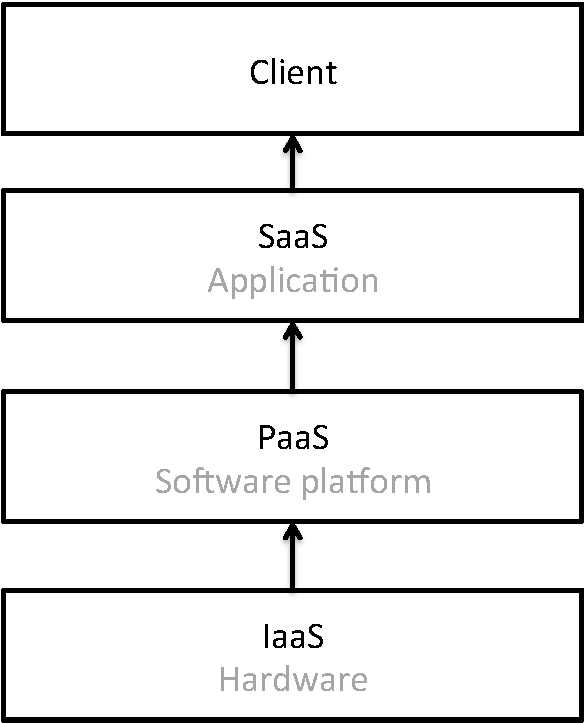
\includegraphics[width=4cm]{img/cloud_models.pdf}
\caption{the relationship of different cloud models}
\label{background:cloud models}
\end{figure}

Cloud computing refers to a model that cloud vendors provide user IT resources and charge them for
the resources they used.
Cloud vendors can offer hardware resources including CPU, memory, hard disk, network and software
resources OS, software suits and applications.
Cloud computing majorly can be classified into following three kinds of models:
\begin{enumerate}
  \item Infrastructure as a service (IaaS): cloud vendors provide only raw machines(physical or
  virtual machine), user need to set up the whole software environment including OS.
  \item Platform as a service (PaaS): in this model, cloud vendors provide hardware as well as
  software platform. Users can use it as a common computer and run applications on the platform.
  Amazon EC2 provides PaaS.
  \item Software as a service (SaaS): Cloud vendors provide a certain applications. Users don't need
  to configure the software themselves.
\end{enumerate}
The relationship of different cloud models can be shown as Figure~.\ref{background:cloud models}

Cloud computing can have following benefits:
\begin{itemize}
  \item User don't need to care about the machine placement and maintenance.
  \item User don't need a large number of machines to meet a temporally request peek and idle for
  the other time, Since cloud instances can set up in a few minutes when the request peek occurs.
  \item User don't need to pay for expensive hardware and software, they just need to pay for what
  they used.
\end{itemize}

\subsection{burst buffer}
\begin{figure}
\centering
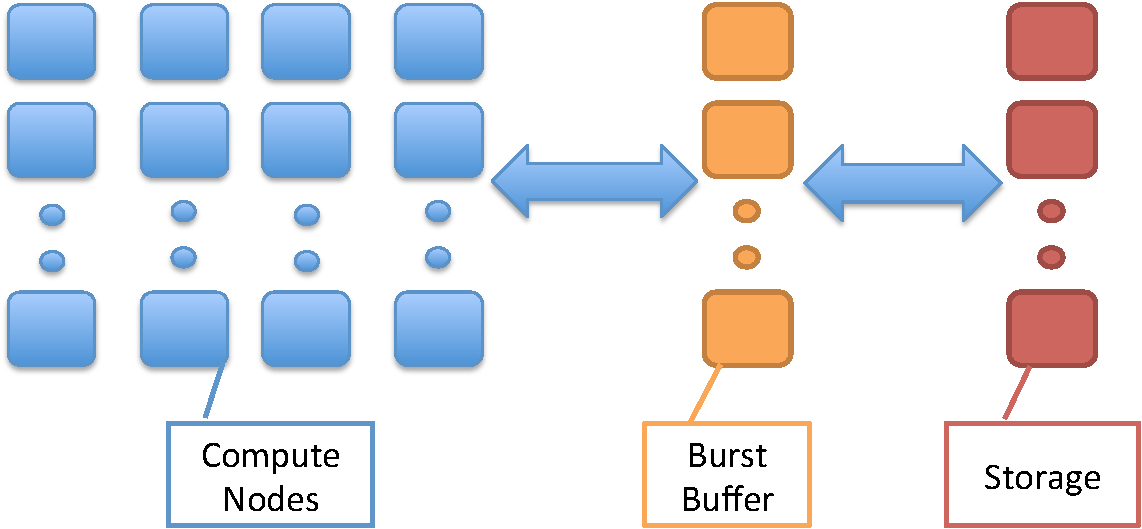
\includegraphics[width=8cm]{img/burst_buffer.pdf}
\caption{burst buffer architecture}
\label{background:burst buffer architecture}
\end{figure}

Modern high performance systems consist of thousands of compute nodes, and hundreds of
applications are running at the same time, some I/O request peak can hardly be meet by current
storage hierarchy. 
Traditional approach which solve such problem by providing a higher bandwidth storage will cause
the storage system underutilization.
Previous research\cite{on_the_role_of_burst_buffers} proposed a
burst buffer system as a new tier of current storage hierarchy.
Burst buffer system use several local compute nodes as a burst buffer to absorb I/O
request. 
Figure~.\ref{background:burst buffer architecture} shows the architecture of burst buffer.

Such burst buffer system can burst the application which has a high data locality I/O pattern, since
the data can be read once from storage and then buffered in the burst buffer system, subsequent
request for the same data can be accessed from burst buffer.
Furthermore, applications which write a lot also can benefit from burst buffer system, by buffering
output data in burst buffer, application can go ahead without waiting data be finally write to
storage.


